\documentclass[11pt,a4paper]{article}
\usepackage[T1]{fontenc}
\usepackage[utf8]{inputenc}
\usepackage{lmodern}
\usepackage[margin=2.0cm]{geometry}
\usepackage{amsmath,amssymb,amsthm,mathtools}
\usepackage{booktabs}
\usepackage{array}
\usepackage{graphicx}
\usepackage{xcolor}
\usepackage{hyperref}

\renewcommand{\abstractname}{\"Osszefoglal\'o}
\renewcommand{\figurename}{\'Abra}
\renewcommand{\tablename}{T\'abl\'azat}
\renewcommand{\refname}{Irodalomjegyz\'ek}

\hypersetup{
    colorlinks=true,
    linkcolor=blue!70!black,
    citecolor=blue!70!black,
    urlcolor=blue!70!black
}

\title{\"Ureg-t\'erfogatar\'annyal s\'ulyozott optikai t\'avols\'agok tesztel\'ese a \texttt{DESI} BAO, a t\"om\"or\'itett \texttt{Planck} CMB \'es n\'egy Ia t\'ipus\'u szupern\'ova-katal\'ogus alapj\'an}

\author{Jozsef Olcsak\\[0.25em]
\small F\"uggetlen kutat\'o $\cdot$ ORCID: \href{https://orcid.org/0009-0003-7311-6522}{0009-0003-7311-6522}\\
\small K\'od- \'es adatarch\'ivum: \href{https://doi.org/10.5281/zenodo.24354218}{doi:10.5281/zenodo.24354218}}
\date{2026.\ november 19.}

\begin{document}
\maketitle

\begin{abstract}
\noindent Az Ia t\'ipus\'u szupern\'ov\'akat (SNe~Ia), a barionikus akusztikus oszcill\'aci\'okat (BAO) \'es a kozmikus mikrohull\'am\'u h\'att\'ersug\'arz\'as (CMB) t\'avols\'ag-priorjait egyes\'it\H{o} k\'es\H{o}i kozmol\'ogiai illeszt\'esek $2{,}5\text{--}4{,}2\sigma$-os preferenci\'at mutatnak az id\H{o}ben v\'altoz\'o s\"ot\'et energia ($w_0 > -1$, $w_a < 0$) ir\'any\'aba, amelynek er\H{o}ss\'ege a szupern\'ova-mint\'ak magasabb anyags\H{u}r\H{u}s\'ege ($\Omega_{m,0} \simeq 0{,}33\text{--}0{,}36$) \'es a BAO+CMB alacsonyabb \'ert\'eke ($\Omega_{m,0} \simeq 0{,}30$) k\"oz\"otti fesz\"ults\'egt\H{o}l f\"ugg. Az inhomog\'en \'ora-dresszing (\textit{Timescape}) modellek alapj\'an --- amelyekben a kozmikus \"uregekben gyorsabban j\'ar\'o saj\'at\'or\'ak ($\mathrm{d}\tau/\mathrm{d}t > 1$) l\'atsz\'olagos $w_0^{\mathrm{app}} > -1$ eltol\'od\'ast keltenek a homog\'en FLRW-sablonokban --- egy 1 szabad param\'eteres fenomenologikus tranzitt\"orv\'enyt ($k = 5$, egyetlen szabad $\alpha \in [0,1]$ s\'uly a s\'ik $\Lambda$CDM felett) vizsg\'alunk, amelyben a dressed Wiltshire-t\'avols\'agderiv\'altat a norm\'alt \"ureg-t\'erfogatar\'any $\alpha_{\mathrm{eff}}(z) = \alpha\,f_v(z)/f_{v,0}$ s\'ulyozza, \'igy a hat\'as a szerkezetk\'epz\H{o}d\'es el\H{o}tt ($z \to z_* \simeq 1090$) automatikusan elt\H{u}nik. M\'ig a konstans s\'ulyoz\'ast ($p = 0$) $\mathcal{O}(0{,}4)$ amplit\'ud\'on\'al kiz\'arja a BAO \'es a t\"om\"or\'itett \texttt{Planck} 2018 $(\omega_b, \omega_c, 100\theta_*)$ prior ($\Delta\chi^2 > +115$), az \"ureg-t\'erfogatar\'annyal s\'ulyozott t\"orv\'eny ($p = 1$) egym\'assal konzisztens $\hat{\alpha}$ becsl\'eseket \'es szignifik\'ans javul\'ast ad mind a n\'egy nyilv\'anos SN~Ia katal\'oguson (\texttt{DESI} BAO + \texttt{Planck} 2018 mellett): $\hat{\alpha} = 0{,}422 \pm 0{,}127$ ($\Delta\chi^2 = -10{,}96$, $\Delta\mathrm{AIC} = -8{,}96$, $\Delta\mathrm{BIC} = -3{,}59$) a \texttt{Pantheon+}, $\hat{\alpha} = 0{,}432 \pm 0{,}122$ ($\Delta\chi^2 = -12{,}66$, $\Delta\mathrm{BIC} = -5{,}14$) az \'ujrakalibr\'alt \texttt{DES-Dovekie}, $\hat{\alpha} = 0{,}545 \pm 0{,}121$ ($\Delta\chi^2 = -20{,}30$, $\Delta\mathrm{BIC} = -12{,}78$) a \texttt{DES-SN5YR}, \'es $\hat{\alpha} = 0{,}594 \pm 0{,}141$ ($\Delta\chi^2 = -15{,}15$, $\Delta\mathrm{BIC} = -11{,}51$) a \texttt{Union3} mint\'an (Chen--Huang--Wang $(R, \ell_A, \omega_b)$ priorral: $\Delta\chi^2 = -9{,}49 \dots -18{,}51$). Az 1-param\'eteres modell mind a n\'egy adatsoron $|\Delta\chi^2| \le 2{,}1$-en bel\"ul el\'eri a 2-param\'eteres CPL ($k = 6$) modell $\chi^2$-\'ert\'ek\'et eggyel kevesebb szabad param\'eterrel ($\Delta\mathrm{BIC} = -3{,}76 \dots -9{,}51$ a CPL-hez k\'epest). A \texttt{Pantheon+} $N = 311$ l\'at\'oir\'any\'at egzakt 1D h\'ur-uni\'o sug\'ark\"ovet\'essel keresztkorrel\'alva az \texttt{SDSS} DR7 3D \texttt{VoidFinder} katal\'ogussal ($z \le 0{,}105$), a v\"or\"oseltol\'od\'asra detrendelt meredeks\'eg $\mathrm{d}\Delta\mu/\mathrm{d}f_{v,\mathrm{LOS}} = -0{,}058 \pm 0{,}036\;\mathrm{mag}$ ($-1{,}59\sigma$): el\H{o}jele megegyezik a gyorsabb \"ureg-\'or\'ak j\'oslat\'aval, statisztikailag pedig egyar\'ant konzisztens a kis egyh\'ej\'u elm\'eleti amplit\'ud\'oval ($-0{,}007 \dots -0{,}014\;\mathrm{mag}$) \'es a zajjal, kijel\"olve a \texttt{DESI} \'es az \texttt{Euclid}/\texttt{LSST} $z \le 0{,}7$ tomogr\'afiai tesztj\'et.
\end{abstract}

\section{Bevezet\'es}
A Dark Energy Spectroscopic Instrument (\texttt{DESI}) BAO-m\'er\'eseit \cite{DESI2024VI,DESIDR2_2025}, a \texttt{Planck} CMB-anizotr\'opi\'akat \cite{Planck2018VI} \'es az Ia t\'ipus\'u szupern\'ov\'akat egyes\'it\H{o} elemz\'esek $2{,}5\text{--}4{,}2\sigma$-os elt\'er\'est jeleznek a $w = -1$ kozmol\'ogiai \'alland\'ot\'ol a $w(a) = w_0 + w_a(1 - a)$ ($w_0 > -1$, $w_a < 0$) ir\'any\'aban. A 6 \'eves Dark Energy Survey elemz\'esben \cite{DES2026DynDE} a \texttt{DES} Y6 + \texttt{Planck} CMB kombin\'aci\'o $(w_0, w_a) = (-0{,}82 \pm 0{,}05;\; -0{,}63^{+0{,}21}_{-0{,}18})$ ($\sim 3{,}0\sigma$) eredm\'enyt ad, m\'ig Efstathiou \cite{Efstathiou2025SN} egy $\sim 0{,}04\;\mathrm{mag}$-os alacsony/magas $z$ k\"oz\"otti kalibr\'aci\'os eltol\'od\'ast mutatott ki a 2024-es \texttt{DES-SN5YR} \cite{DESSN5YR2024} \'es a \texttt{Pantheon+} \cite{Brout2022} k\"oz\"ott, ami a \texttt{DES-Dovekie} fotometriai \'ujrakalibr\'aci\'ohoz \cite{PopovicDovekie2025} vezetett a spline-binnelt \texttt{Union3} \cite{RubinUnion3_2025} mellett. Mind a n\'egy nyilv\'anos SN~Ia katal\'oguson a s\'ik $\Lambda$CDM szupern\'ova-illeszt\'es magasabb jelenlegi anyags\H{u}r\H{u}s\'eget prefer\'al --- $\Omega_{m,0} = 0{,}3326 \pm 0{,}0182$ (\texttt{Pantheon+}), $0{,}3303 \pm 0{,}0153$ (\texttt{DES-Dovekie}), $0{,}3520 \pm 0{,}0168$ (\texttt{DES-SN5YR}), illetve $0{,}3559 \pm 0{,}0270$ (\texttt{Union3}) --- mint a \texttt{DESI} BAO + \texttt{Planck} CMB ($\Omega_{m,0} \simeq 0{,}301$).

Alternat\'iv fizikai mechanizmust k\'in\'alnak az inhomog\'en gravit\'aci\'os \'ora-dresszing (\textit{Timescape}) modellek \cite{Wiltshire2009PRD,LaneWiltshire2025MNRAS,SeifertWiltshire2025MNRAS}: mivel a fotonok k\"ot\"ott galaxissz\'alakon ($t_w$) \'es t\'agul\'o kozmikus \"uregeken ($f_v(z)$, gyorsabb $\bar{\gamma} = \mathrm{d}t/\mathrm{d}t_w = 1 + \frac{1}{2}f_v > 1$ \'oraj\'ar\'as) haladnak \'at, az egy\'or\'as s\'ik FLRW-sablon illeszt\'ese s\"ot\'etenergia-folyad\'ek n\'elk\"ul is l\'atsz\'olagos $w_0^{\mathrm{app}} > -1$ \'ert\'eket ad. A standard SALT2 \texttt{Pantheon+} kovarianci\'an azonban a tiszta s\'ulyozatlan Timescape $\chi^2_{\mathrm{SN}} = 1403{,}83$-at ad $f_{v,0} = 0{,}723$-n\'al ($\Delta\chi^2 = +16{,}50$ a $\Lambda$CDM-hez k\'epest; szabad $f_{v,0} = 0{,}853$-n\'al $1391{,}51$), j\'ollehet nyers f\'enyg\"orbe-\'ujrailleszt\'essel kedvez\H{o}bb illeszked\'es \'erhet\H{o} el \cite{LaneWiltshire2025MNRAS,SeifertWiltshire2025MNRAS}.

Ezzel szemben egyetlen \'or\'aj\'u s\'ik $\Lambda$CDM h\'att\'eren Kantowski \cite{Kantowski1969}, Dyer \'es Roeder \cite{DyerRoeder1973}, valamint Weinberg \cite{Weinberg1976} klasszikus eredm\'enye alapj\'an a Sachs-egyenlet Ricci-f\'okusz\'al\'asi t\'enyez\H{o}j\'enek ($\alpha_{\mathrm{beam}}(z)$) m\'odos\'it\'asa nem v\'altoztatja meg $D_A''(0) = -(2 + \frac{3}{2}\Omega_{m,0})\frac{c}{H_0}$ \'ert\'ek\'et ($D_A(0) = 0$ miatt), \'igy $w_0^{\mathrm{app}}(z \to 0) = -1$ azonoss\'agszer\H{u}en megmarad, a gyenge t\'erbeli \"uregpotenci\'alok ($|\Phi|/c^2 \lesssim 5\times 10^{-4}$) pedig $< 10^{-3}$-tal m\'odos\'itj\'ak $w_0^{\mathrm{app}}$-t.

Tanulm\'anyunkban egy 1-param\'eteres fenomenologikus, \"ureg-t\'erfogatar\'annyal s\'ulyozott tranzitt\"orv\'enyt vizsg\'alunk szigor\'u $k = 5$ param\'etersz\'aml\'al\'assal mind a n\'egy nyilv\'anos SN~Ia katal\'oguson (\texttt{DESI} BAO + t\"om\"or\'itett \texttt{Planck} 2018 CMB mellett), megvizsg\'aljuk az $f_{v,0}$- \'es $H_0$-norm\'al\'asi \'erz\'ekenys\'eget, majd elv\'egezz\"uk a \texttt{Pantheon+} \'es az \texttt{SDSS} DR7 3D \texttt{VoidFinder} katal\'ogus \cite{Douglass2023ApJS} k\"ozvetlen sug\'ark\"ovet\'eses keresztkorrel\'aci\'oj\'at.

\section{Fenomenologikus \"ureg-t\'erfogatar\'annyal s\'ulyozott t\'avols\'agmodell}
A Buchert--Wiltshire trackerben \cite{Wiltshire2009PRD,LaneWiltshire2025MNRAS} a dressed t\'avols\'ag z\'art alakja $D_{\mathrm{TS}}(z) = (1+z)d_A^{\mathrm{TS}}(z)$, ahol
\begin{equation}
\begin{split}
    \bar{H}_0 d_A^{\mathrm{TS}}(z) &= c\,x(z)^{2/3}\bigl[\mathcal{F}(x_0) - \mathcal{F}(x(z))\bigr], \\
    \mathcal{F}(x) &= 2x^{1/3} + \frac{b^{1/3}}{6}\ln\frac{(x^{1/3}+b^{1/3})^2}{x^{2/3}-b^{1/3}x^{1/3}+b^{2/3}} + \frac{b^{1/3}}{\sqrt{3}}\arctan\frac{2x^{1/3}-b^{1/3}}{\sqrt{3}\,b^{1/3}},
\end{split}
\label{eq:wiltshire-exact}
\end{equation}
$x_0 = \frac{2+f_{v,0}}{3}$, $b = \frac{2(1-f_{v,0})(2+f_{v,0})}{9f_{v,0}}$, $\frac{H_0^{\mathrm{TS}}}{\bar{H}_0} = \frac{4f_{v,0}^2 + f_{v,0} + 4}{2(2+f_{v,0})}$, \'es $1 + z = \frac{2 + f_v}{2 + f_{v,0}}\bigl(\frac{f_{v,0}}{f_v}\bigr)^{2/3}\frac{1 - f_v}{1 - f_{v,0}}$, \'igy a korai univerzumban $f_v(z) \propto (1+z)^{-1} \to 0$ ($f_v(z_*) \approx 2{,}2\times 10^{-3}$). Alapkalibr\'aci\'onkban (\texttt{H1}) a fal-keretbeli gyorsul\'asi gy\"ok\"ot ($q_{\mathrm{wall}}(f_{\mathrm{acc}}) = 0 \implies f_{\mathrm{acc}} = 0{,}586708$) a $\Lambda$CDM $z_{\mathrm{acc}} = [2(1-\Omega_{m,0})/\Omega_{m,0}]^{1/3} - 1$ v\"or\"oseltol\'od\'ashoz illesztj\"uk ($\Omega_{m,0} = 0{,}3153 \mapsto f_{v,0} = 0{,}7234$), \'am a \ref{tab:chw-fv0}.\ t\'abl\'azatban \texttt{H1} n\'elk\"ul, r\"ogz\'itett $f_{v,0} \in [0{,}65; 0{,}80]$ \'ert\'ekeken is ellen\H{o}rizz\"uk az eredm\'eny robusztuss\'ag\'at.

A dimenzi\'omentes $\tilde{D}_{\mathrm{TS}}(z) := H_0^{\mathrm{TS}} D_{\mathrm{TS}}(z)/c$ ($\tilde{D}_{\mathrm{TS}}'(0) = 1$) \'es $D_{\mathrm{hor}}(z) = \int_0^z E_{\mathrm{hor}}(z')^{-1}\mathrm{d}z'$ kombin\'aci\'oj\'at egyetlen szabad $\alpha \in [0, 1]$ param\'eteres fenomenologikus modellk\'ent vizsg\'aljuk:
\begin{enumerate}
    \item \textit{Konstans s\'uly\'u ansatz} (\texttt{H2a}, $p = 0$): $\tilde{D}_{\mathrm{obs}}(z) = (1 - \alpha)D_{\mathrm{hor}}(z) + \alpha \tilde{D}_{\mathrm{TS}}(z)$ minden $z$-n (m\'eg $z_* \simeq 1090$-n\'el is).
    \item \textit{\"Ureg-t\'erfogatar\'annyal s\'ulyozott tranzitt\"orv\'eny} (\texttt{H2-vol}, $p = 1$) \'es \textit{csatolt Sachs-ODE} (\texttt{Forward H2-Sachs}, $p = 1$): $\alpha_{\mathrm{eff}}(z) := \alpha\,\frac{f_v(z)}{f_{v,0}}$ s\'ulyoz\'assal ($z \to z_*$ hat\'aresetben automatikusan elt\H{u}nik):
    \begin{equation}
        \frac{\mathrm{d}\tilde{D}_{\mathrm{obs}}^{\mathrm{(H2\text{-}vol)}}}{\mathrm{d}z} = \frac{1 - \alpha_{\mathrm{eff}}(z)}{E_{\mathrm{hor}}(z)} + \alpha_{\mathrm{eff}}(z)\frac{\mathrm{d}\tilde{D}_{\mathrm{TS}}}{\mathrm{d}z}, \qquad D_M^{\mathrm{obs}}(z) = \frac{c}{H_0}\tilde{D}_{\mathrm{obs}}(z),
        \label{eq:h2-vol}
    \end{equation}
    illetve az el\H{o}re ir\'anyul\'o $\frac{\mathrm{d}}{\mathrm{d}z}\bigl[(1+z)^2 E_{\mathrm{ray}}(z)\frac{\mathrm{d}\tilde{D}_A}{\mathrm{d}z}\bigr] + \frac{3}{2}\Omega_{m,0}\frac{(1+z)^3}{E_{\mathrm{ray}}(z)}\tilde{D}_A(z) = 0$ egyenletben.
\end{enumerate}

\paragraph{K\"oz\"os $H_0$-norm\'al\'as \'es $k = 5$ param\'etersz\'aml\'al\'as.} Az \eqref{eq:h2-vol} t\"orv\'enyben mindk\'et \'ag ugyanazzal a $H_0 = 100h\;\mathrm{km\,s^{-1}\,Mpc^{-1}}$ jelenlegi Hubble-norm\'al\'assal szerepel ($\tilde{D}_{\mathrm{obs}}'(0) = 1$), m\'ig $r_d$ \'es $r_s(z_*)$ a korai FLRW-h\'att\'erb\H{o}l ad\'odik; ha ehelyett a norm\'alatlan bare $\mathrm{d}(\bar{H}_0 D_{\mathrm{TS}}/c)/\mathrm{d}z$ meredeks\'eget keverj\"uk ($\bar{H}_0/H_0^{\mathrm{TS}} \simeq 0{,}749$), a BAO+CMB illeszt\'es $\hat{\alpha} = 0{,}000 \pm 0{,}043$-ra szor\'itja a s\'ulyt. Mivel a $p = 1$ s\'ulyoz\'ast a $p = 0$ modell korai univerzumos kudarca ut\'an v\'alasztottuk, a \texttt{H2-vol} \'es a \texttt{Forward H2-Sachs} szigor\'uan $k = 5$ szabad param\'eteres modell ($h, \omega_b, \omega_c, M_B, \alpha$; $\Delta k = +1$ a $\Lambda$CDM-hez \'es $\Delta k = -1$ a $k = 6$ CPL-hez k\'epest).

\section{Adatsorok, t\"obbkatal\'ogusos eredm\'enyek \'es 3D l\'at\'oir\'any-teszt}
Az \"on\'all\'o \texttt{NumPy}/\texttt{SciPy} csomag (\texttt{verify\_C9}, $\sim 35\;\mathrm{s}$ fut\'asid\H{o}) BDF2 \texttt{RECFAST}~v1.5 rekombin\'aci\'ot \'es Fermi--Dirac neutr\'in\'ointegr\'alt ($\sum m_\nu = 0{,}06\;\mathrm{eV}$) haszn\'al n\'egy nyilv\'anos SN~Ia katal\'oguson (\texttt{Pantheon+} $N=1580$ \cite{Brout2022}, \'ujrakalibr\'alt \texttt{DES-Dovekie} $N=1820$ \cite{PopovicDovekie2025}, \texttt{DES-SN5YR} $N=1829$ \cite{DESSN5YR2024}, \texttt{Union3} $N=22$ spline-csom\'opont \cite{RubinUnion3_2025}), a 13-pontos \texttt{DESI} BAO-n \cite{DESI2024VI,DESIDR2_2025} \'es a \texttt{Planck} 2018 \texttt{TT,TE,EE+lowE} $3\times 3$-as $(\omega_b, \omega_c, 100\theta_*)$ MCMC kovarianci\'aj\'an \cite{Planck2018VI} (keresztellen\H{o}rz\'esk\'ent a Chen--Huang--Wang \cite{ChenHuangWang2019} $(R, \ell_A, \omega_b)$ priorral \'es a 15 Moresco kozmikus kronom\'eterrel \cite{Moresco2020}).

\begin{figure}[ht!]
    \centering
    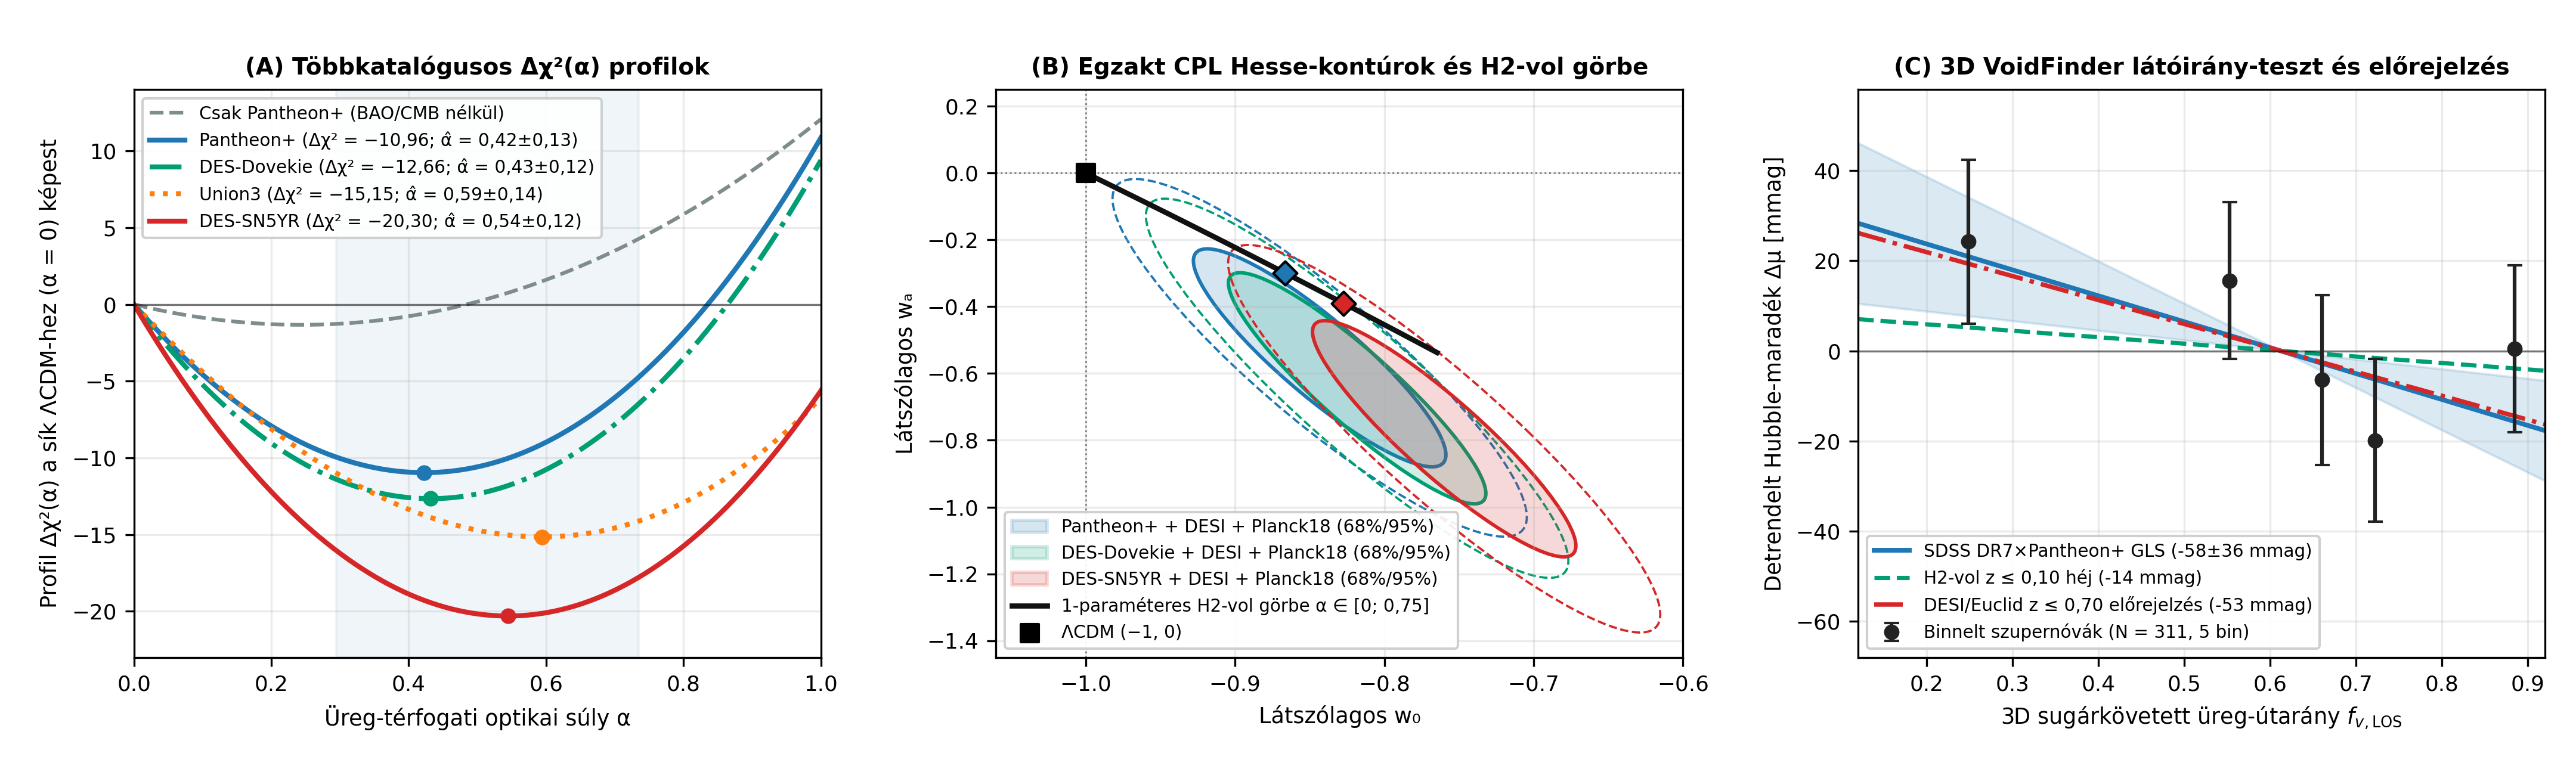
\includegraphics[width=0.99\textwidth]{fig_sub4_void_clock_des2026_and_galactic_dip_hu.png}
    \caption{(A) A \texttt{H2-vol} ($p=1$) profil $\Delta\chi^2(\alpha)$ g\"orb\'ei mind a n\'egy SN~Ia katal\'oguson (\texttt{DESI} BAO + \texttt{Planck} 2018 mellett) a lapos \texttt{Pantheon+}-only g\"orb\'evel (szaggatott sz\"urke) szemben; (B) az egzakt $5\times 5$ Hesse-m\'atrixb\'ol sz\'amolt $68\%/95\%$-os CPL kont\'urok \'es az 1-param\'eteres \texttt{H2-vol} l\'atsz\'olagos $(w_0^{\mathrm{app}}, w_a^{\mathrm{app}})$ g\"orb\'eje; (C) $N = 311$ \texttt{Pantheon+} l\'at\'oir\'any 3D sug\'ark\"ovet\'ese az \texttt{SDSS} DR7 \texttt{VoidFinder} katal\'oguson \cite{Douglass2023ApJS} kereszt\"ul ($-58 \pm 36\;\mathrm{mmag}$ empirikus GLS s\'av, $-14\;\mathrm{mmag}$ $z \le 0{,}10$ elm\'eleti h\'ej, \'es $-53\;\mathrm{mmag}$ $z \le 0{,}70$ \texttt{DESI}/\texttt{Euclid} el\H{o}rejelz\'es).}
    \label{fig:v7-main}
\end{figure}

\begin{table}[ht!]
\centering
\scriptsize
\setlength{\tabcolsep}{3.0pt}
\renewcommand{\arraystretch}{1.13}
\resizebox{\textwidth}{!}{%
\begin{tabular}{llcccccccc}
\toprule
SN~Ia katal\'ogus (+ \texttt{DESI} BAO + \texttt{Planck18}) & Modell & $k$ & Optimum $(H_0,\;\Omega_{m,0})$ & $\hat{\alpha} \pm \sigma_\alpha$ vagy $(w_0,\;w_a)$ & $\chi^2_{\mathrm{SN}}$ / $\chi^2_{\mathrm{BAO}}$ / $\chi^2_{\mathrm{CMB}}$ & $\chi^2_{\mathrm{tot}}$ & $\Delta\chi^2$ vs.\ $\Lambda$CDM ($1\mathrm{dof}\;\sigma$) & $\Delta\mathrm{AIC}$ / $\Delta\mathrm{BIC}$ vs.\ $\Lambda$CDM & $\Delta\mathrm{BIC}$ vs.\ CPL \\
\midrule
\texttt{Pantheon+} ($N_{\mathrm{SN}}=1580$, $N_{\mathrm{tot}}=1596$) & S\'ik $\Lambda$CDM (\texttt{M0}) & $4$ & $(68{,}42;\;0{,}3009)$ & $\alpha \equiv 0$ & $1389{,}56$ / $13{,}31$ / $4{,}09$ & $1406{,}97$ & $0{,}00$ (---) & $0{,}00$ / $0{,}00$ & $-5{,}92$ \\
 & \texttt{H2-vol} ($p=1$, \"ureg-s\'ulyozott) & $5$ & $(67{,}32;\;0{,}3138)$ & $0{,}422 \pm 0{,}127$ & $1386{,}64$ / $8{,}82$ / $0{,}55$ & $1396{,}01$ & $-10{,}96$ ($3{,}31\sigma$) & $-8{,}96$ / $-3{,}59$ & $-9{,}51$ \\
 & \texttt{Forward H2-Sachs} ($p=1$) & $5$ & $(67{,}39;\;0{,}3121)$ & $0{,}471 \pm 0{,}151$ & $1386{,}47$ / $9{,}20$ / $1{,}43$ & $1397{,}10$ & $-9{,}87$ ($3{,}14\sigma$) & $-7{,}87$ / $-2{,}49$ & $-8{,}42$ \\
 & Szabad CPL (\texttt{M1b}, Hesse) & $6$ & $(67{,}61;\;0{,}3103)$ & $(-0{,}843\pm 0{,}056;\;-0{,}553\pm 0{,}215)$ & $1386{,}53$ / $10{,}36$ / $1{,}26$ & $1398{,}14$ & $-8{,}83$ (---) & $-4{,}83$ / $+5{,}92$ & $0{,}00$ \\
 & Tiszta Timescape ($\alpha=1$) & $4$ & $(66{,}54;\;0{,}3273)$ & $\alpha \equiv 1$ & $1400{,}62$ / $14{,}08$ / $3{,}13$ & $1417{,}82$ & $+10{,}85$ (---) & $+10{,}85$ / $+10{,}85$ & $+4{,}93$ \\
\midrule
\texttt{DES-Dovekie} ($N_{\mathrm{SN}}=1820$, $N_{\mathrm{tot}}=1836$) & S\'ik $\Lambda$CDM (\texttt{M0}) & $4$ & $(68{,}39;\;0{,}3013)$ & $\alpha \equiv 0$ & $1635{,}19$ / $13{,}65$ / $3{,}85$ & $1652{,}70$ & $0{,}00$ (---) & $0{,}00$ / $0{,}00$ & $-3{,}06$ \\
 & \texttt{H2-vol} ($p=1$, \"ureg-s\'ulyozott) & $5$ & $(67{,}31;\;0{,}3139)$ & $0{,}432 \pm 0{,}122$ & $1630{,}75$ / $8{,}76$ / $0{,}53$ & $1640{,}04$ & $-12{,}66$ ($3{,}56\sigma$) & $-10{,}66$ / $-5{,}14$ & $-8{,}20$ \\
 & \texttt{Forward H2-Sachs} ($p=1$) & $5$ & $(67{,}32;\;0{,}3129)$ & $0{,}509 \pm 0{,}148$ & $1630{,}12$ / $9{,}13$ / $1{,}28$ & $1640{,}52$ & $-12{,}18$ ($3{,}49\sigma$) & $-10{,}18$ / $-4{,}66$ & $-7{,}72$ \\
 & Szabad CPL (\texttt{M1b}, Hesse) & $6$ & $(67{,}48;\;0{,}3118)$ & $(-0{,}818\pm 0{,}057;\;-0{,}644\pm 0{,}228)$ & $1629{,}47$ / $10{,}30$ / $0{,}96$ & $1640{,}72$ & $-11{,}98$ (---) & $-7{,}98$ / $+3{,}06$ & $0{,}00$ \\
\midrule
\texttt{DES-SN5YR} ($N_{\mathrm{SN}}=1829$, $N_{\mathrm{tot}}=1845$) & S\'ik $\Lambda$CDM (\texttt{M0}) & $4$ & $(68{,}32;\;0{,}3022)$ & $\alpha \equiv 0$ & $1649{,}46$ / $14{,}40$ / $3{,}40$ & $1667{,}25$ & $0{,}00$ (---) & $0{,}00$ / $0{,}00$ & $+4{,}35$ \\
 & \texttt{H2-vol} ($p=1$, \"ureg-s\'ulyozott) & $5$ & $(67{,}07;\;0{,}3175)$ & $0{,}545 \pm 0{,}121$ & $1638{,}29$ / $8{,}63$ / $0{,}03$ & $1646{,}95$ & $-20{,}30$ ($4{,}51\sigma$) & $-18{,}30$ / $-12{,}78$ & $-8{,}43$ \\
 & \texttt{Forward H2-Sachs} ($p=1$) & $5$ & $(67{,}04;\;0{,}3164)$ & $0{,}644 \pm 0{,}148$ & $1637{,}75$ / $9{,}45$ / $0{,}59$ & $1647{,}79$ & $-19{,}46$ ($4{,}41\sigma$) & $-17{,}46$ / $-11{,}94$ & $-7{,}59$ \\
 & Szabad CPL (\texttt{M1b}, Hesse) & $6$ & $(66{,}87;\;0{,}3177)$ & $(-0{,}760\pm 0{,}058;\;-0{,}796\pm 0{,}233)$ & $1637{,}56$ / $9{,}50$ / $0{,}80$ & $1647{,}87$ & $-19{,}39$ (---) & $-15{,}39$ / $-4{,}35$ & $0{,}00$ \\
\midrule
\texttt{Union3} ($N_{\mathrm{bins}}=22$, $N_{\mathrm{tot}}=38$) & S\'ik $\Lambda$CDM (\texttt{M0}) & $4$ & $(68{,}44;\;0{,}3007)$ & $\alpha \equiv 0$ & $28{,}54$ / $13{,}16$ / $4{,}21$ & $45{,}90$ & $0{,}00$ (---) & $0{,}00$ / $0{,}00$ & $+7{,}75$ \\
 & \texttt{H2-vol} ($p=1$, \"ureg-s\'ulyozott) & $5$ & $(66{,}98;\;0{,}3189)$ & $0{,}594 \pm 0{,}141$ & $22{,}07$ / $8{,}68$ / $0{,}00$ & $30{,}76$ & $-15{,}15$ ($3{,}89\sigma$) & $-13{,}15$ / $-11{,}51$ & $-3{,}76$ \\
 & \texttt{Forward H2-Sachs} ($p=1$) & $5$ & $(66{,}94;\;0{,}3177)$ & $0{,}699 \pm 0{,}179$ & $21{,}77$ / $9{,}73$ / $0{,}40$ & $31{,}90$ & $-14{,}00$ ($3{,}74\sigma$) & $-12{,}00$ / $-10{,}37$ & $-2{,}61$ \\
 & Szabad CPL (\texttt{M1b}, Hesse) & $6$ & $(66{,}07;\;0{,}3258)$ & $(-0{,}678\pm 0{,}091;\;-1{,}014\pm 0{,}308)$ & $21{,}59$ / $8{,}68$ / $0{,}61$ & $30{,}88$ & $-15{,}03$ (---) & $-11{,}03$ / $-7{,}75$ & $0{,}00$ \\
\bottomrule
\end{tabular}%
}
\caption{K\"ozvetlen t\"obbpr\'ob\'as illeszt\'esek mind a n\'egy nyilv\'anos SN~Ia katal\'oguson a \texttt{DESI} 13-pontos BAO \'es a t\"om\"or\'itett \texttt{Planck} 2018 $3\times 3$ $(\omega_b, \omega_c, 100\theta_*)$ MCMC prior mellett (\texttt{verify\_C9}, \H{o}szinte $k=5$ param\'etersz\'aml\'al\'assal). Konstans s\'uly\'u \texttt{H2a} ($p=0$) $\alpha = \hat{\alpha}_{p=1}$-n\'el $\Delta\chi^2 = +115{,}4 \dots +264{,}5$-tel kiz\'art.}
\label{tab:multi-sn}
\end{table}

\begin{table}[ht!]
\centering
\scriptsize
\setlength{\tabcolsep}{4.0pt}
\renewcommand{\arraystretch}{1.12}
\resizebox{\textwidth}{!}{%
\begin{tabular}{lcccc|ccccc}
\toprule
 & \multicolumn{4}{c|}{\texttt{Chen--Huang--Wang (2019)} $(R,\ell_A,\omega_b)$ CMB prior ($k=5$ \texttt{H2-vol})} & \multicolumn{5}{c}{Fix-$f_{v,0}$ \'erz\'ekenys\'eg \texttt{H1} n\'elk\"ul (\texttt{Pantheon++DESI+Planck18})} \\
Mutat\'o & \texttt{Pantheon+} & \texttt{DES-Dovekie} & \texttt{DES-SN5YR} & \texttt{Union3} & $f_{v,0}=0{,}650$ & $f_{v,0}=0{,}695$ & $f_{v,0}=0{,}724$ (\texttt{H1}) & $f_{v,0}=0{,}762$ \cite{Wiltshire2009PRD} & $f_{v,0}=0{,}800$ \\
\midrule
$\hat{\alpha} \pm \sigma_\alpha$ & $0{,}398 \pm 0{,}130$ & $0{,}409 \pm 0{,}125$ & $0{,}529 \pm 0{,}124$ & $0{,}580 \pm 0{,}149$ & $0{,}058 \pm 0{,}090$ & $0{,}351 \pm 0{,}182$ & $0{,}431 \pm 0{,}122$ & $0{,}259 \pm 0{,}074$ & $0{,}137 \pm 0{,}044$ \\
$\Delta\chi^2$ vs.\ $\Lambda$CDM & $-9{,}49$ ($3{,}08\sigma$) & $-11{,}11$ ($3{,}33\sigma$) & $-18{,}51$ ($4{,}30\sigma$) & $-13{,}43$ ($3{,}66\sigma$) & $-0{,}43$ & $-4{,}81$ & $-10{,}98$ & $-11{,}27$ & $-9{,}39$ \\
$\Delta\mathrm{BIC}$ vs.\ $\Lambda$CDM / CPL & $-2{,}11$ / $-8{,}97$ & $-3{,}59$ / $-7{,}71$ & $-10{,}99$ / $-7{,}82$ & $-9{,}79$ / $-3{,}18$ & $+6{,}94$ & $+2{,}56$ & $-3{,}61$ & $-3{,}89$ & $-2{,}01$ \\
\bottomrule
\end{tabular}%
}
\caption{Balra: \texttt{H2-vol} ($p=1$, $k=5$) keresztellen\H{o}rz\'es a Chen--Huang--Wang \cite{ChenHuangWang2019} $(R, \ell_A, \omega_b)$ priorral. Jobbra: \'erz\'ekenys\'eg fix $f_{v,0} \in [0{,}65; 0{,}80]$ \'ert\'ekekre a \texttt{H1} kalibr\'aci\'o felt\'etelez\'ese n\'elk\"ul.}
\label{tab:chw-fv0}
\end{table}

\begin{enumerate}
    \item \textit{T\"obbkatal\'ogusos konkordancia (\ref{fig:v7-main}A--B.\ \'abra, \ref{tab:multi-sn}--\ref{tab:chw-fv0}.\ t\'abl\'azat):} M\'ig puszt\'an a \texttt{Pantheon+} szupern\'ov\'akon az $\alpha \in [0; 0{,}43]$ s\'av lapos az $\Omega_{m,0}$-eltol\'assal val\'o degener\'aci\'o miatt, a \texttt{DESI} BAO \'es a t\"om\"or\'itett \texttt{Planck} 2018 prior bevon\'asa mind a n\'egy mint\'an egym\'assal $<1\sigma$-n bel\"ul egyez\H{o} $\hat{\alpha} \in [0{,}42; 0{,}59]$ optimumot \'es negat\'iv $\Delta\mathrm{AIC}$ / $\Delta\mathrm{BIC}$ \'ert\'ekeket ad ($\Delta\chi^2 = -10{,}96$ \texttt{Pantheon+}, $-12{,}66$ \texttt{DES-Dovekie}, $-20{,}30$ \texttt{DES-SN5YR}, $-15{,}15$ \texttt{Union3}; diagon\'alis $\theta_*+\mathrm{BBN}+\omega_c+\mathrm{CC15}$ ellen\H{o}rz\'es: $\chi^2_{\Lambda\mathrm{CDM}} = 1413{,}85$, $\Delta\chi^2 = -11{,}31$, $\hat{\alpha} = 0{,}425 \pm 0{,}125$). A \texttt{DES-Dovekie} + \texttt{DESI} + \texttt{Planck18} szabad CPL illeszt\'es $(-0{,}818 \pm 0{,}057;\; -0{,}644 \pm 0{,}228)$ k\"ozvetlen\"ul reproduk\'alja a \texttt{DES} Y6 + CMB eredm\'enyt \cite{DES2026DynDE}.
    \item \textit{3D \texttt{SDSS} DR7 \texttt{VoidFinder} sug\'ark\"ovet\'eses l\'at\'oir\'any-teszt (\ref{fig:v7-main}C.\ \'abra):} Az \'eszaki galaktikus sapka bels\H{o} tartom\'any\'aban fekv\H{o} $N = 311$ \texttt{Pantheon+} szupern\'ova f\'eny\'utj\'at egzakt 1D h\'ur-uni\'oval \'atk\"ovetve a $39\,735$ \texttt{Planck} 2018 koordin\'at\'aj\'u 3D \texttt{VoidFinder} g\"omb\"on \cite{Douglass2023ApJS}, a t\'erfogaton bel\"uli ($0{,}02 \le z \le 0{,}105$, $N = 151$) minta $\mathrm{d}\Delta\mu/\mathrm{d}f_{v,\mathrm{LOS}} = -0{,}093 \pm 0{,}066\;\mathrm{mag}$ ($-1{,}41\sigma$, \'egbolt-permut\'aci\'os $p = 0{,}106$), a $[30, 300]\,h^{-1}\,\mathrm{Mpc}$ el\H{o}t\'erh\'ej m\"og\"otti ($z > 0{,}11$, $N = 160$) minta $-0{,}040 \pm 0{,}044\;\mathrm{mag}$ ($-0{,}92\sigma$, $p = 0{,}387$), az egyes\'itett $N = 311$ minta pedig $-0{,}058 \pm 0{,}036\;\mathrm{mag}$ ($-1{,}59\sigma$) meredeks\'eget ad. Ez az el\H{o}jel megegyezik az \"ureg-\'or\'ak j\'oslat\'aval ($\Delta\mu < 0$), \'am $z_{\mathrm{void}} \le 0{,}105$ m\'elys\'egn\'el egyar\'ant konzisztens a kis egyh\'ej\'u elm\'eleti v\'arhat\'o \'ert\'ekkel ($-0{,}007 \dots -0{,}014\;\mathrm{mag}$) \'es a statisztikai zajjal; a $z \le 0{,}70$-ig terjed\H{o} \texttt{DESI} + \texttt{Euclid}/\texttt{LSST} 3D \"uregtomogr\'afia ($-0{,}053\;\mathrm{mag}$ meredeks\'eg, $N_{\mathrm{SN}} \ge 5\,000$) $> 5\sigma$ szignifikanci\'aval d\"ont a modell \'es a homog\'en s\"ot\'et energia k\"oz\"ott.
\end{enumerate}

\section{Konkl\'uzi\'o}
A $z \to z_*$ hat\'aresetben elt\H{u}n\H{o}, 1 szabad param\'eteres ($k = 5$) \"ureg-t\'erfogati s\'ulyoz\'as mind a n\'egy nyilv\'anos szupern\'ova-katal\'oguson feloldja az SN--BAO $\Omega_{m,0}$-fesz\"ults\'eget ($\Delta\chi^2 = -9{,}5 \dots -20{,}3$, $\hat{\alpha} \in [0{,}40; 0{,}59]$), eggyel kevesebb param\'eterrel el\'erve a 2-param\'eteres CPL illeszked\'es\'et ($\Delta\mathrm{BIC} = -3{,}2 \dots -9{,}5$ a CPL-hez k\'epest). Nyitott elm\'eleti feladat az \eqref{eq:h2-vol} t\"orv\'eny levezet\'ese egyetlen inhomog\'en 4D metrika f\'enyk\'up-\'atlagol\'as\'ab\'ol, valamint a $0{,}1 \le z \le 0{,}7$ tartom\'any\'u \texttt{DESI}/\texttt{Euclid} l\'at\'oir\'any-tomogr\'afia v\'egrehajt\'asa.

\paragraph{Adat- \'es k\'odhozz\'af\'erhet\H{o}s\'eg.} {\sloppy Az \"on\'all\'o \texttt{NumPy}/\texttt{SciPy} ellen\H{o}rz\H{o} szkript (\path{verify_C9_void_clock_timescape_apparent_w0_wa_audit.py}, $\sim 35\;\mathrm{s}$ fut\'asid\H{o}, \texttt{-{}-no-asserts} kapcsol\'oval) \'es minden nyers adatsor megtal\'alhat\'o a \path{supplementary_code_and_data/} mapp\'aban \'es a Zenod\'on (\href{https://doi.org/10.5281/zenodo.24354218}{doi:10.5281/zenodo.24354218}).\par}

\begin{thebibliography}{99}
\bibitem{DESI2024VI} A.~G.~Adame \textit{et al.} (DESI Collaboration), \textit{DESI 2024 VI: Cosmological Constraints from the Measurements of Baryon Acoustic Oscillations}, JCAP \textbf{02}, 021 (2025), arXiv:2404.03002.
\bibitem{DESIDR2_2025} DESI Collaboration, \textit{DESI DR2 Results II: Measurements of Baryon Acoustic Oscillations and Cosmological Constraints}, arXiv:2503.14738 (2025).
\bibitem{Planck2018VI} N.~Aghanim \textit{et al.} (Planck Collaboration), \textit{Planck 2018 results. VI. Cosmological parameters}, Astron.\ Astrophys.\ \textbf{641}, A6 (2020), arXiv:1807.06209.
\bibitem{DES2026DynDE} DES Collaboration, \textit{Constraints on Dynamical Dark Energy from Multiple Probes in the Full Dark Energy Survey}, arXiv:2605.27221 (2026).
\bibitem{Efstathiou2025SN} G.~Efstathiou, \textit{Evolving Dark Energy or Supernovae Systematics?}, Mon.\ Not.\ R.\ Astron.\ Soc.\ \textbf{538}, 875 (2025), arXiv:2408.07175.
\bibitem{DESSN5YR2024} M.~Vincenzi \textit{et al.} (DES Collaboration), \textit{The Dark Energy Survey: Cosmology Results with $\sim 1500$ New High-redshift Type Ia Supernovae Using the Full 5 Year Dataset}, Astrophys.\ J.\ Lett.\ \textbf{973}, L14 (2024), arXiv:2401.02929.
\bibitem{Brout2022} D.~Brout \textit{et al.}, \textit{The Pantheon+ Analysis: Cosmological Constraints}, Astrophys.\ J.\ \textbf{938}, 110 (2022), arXiv:2202.04077.
\bibitem{PopovicDovekie2025} B.~Popovic \textit{et al.} (DES Collaboration), \textit{DES-Dovekie Recalibrated Type Ia Supernova Compilation and Covariance Release}, GitHub \texttt{des-science/DES-SN5YR} (2025).
\bibitem{RubinUnion3_2025} D.~Rubin \textit{et al.}, \textit{Union Through UNITY: Cosmology with $2,000$ SNe Using a Unified Bayesian Framework}, Astrophys.\ J.\ (2025), arXiv:2311.12098.
\bibitem{Wiltshire2009PRD} D.~L.~Wiltshire, \textit{Average observational quantities in the timescape cosmology}, Phys.\ Rev.\ D \textbf{80}, 123512 (2009), arXiv:0909.0749.
\bibitem{LaneWiltshire2025MNRAS} Z.~G.~Lane, A.~Seifert, R.~Ridden-Harper, and D.~L.~Wiltshire, \textit{Cosmological foundations revisited with Pantheon+}, Mon.\ Not.\ R.\ Astron.\ Soc.\ \textbf{536}, 1752 (2025), arXiv:2311.01438.
\bibitem{SeifertWiltshire2025MNRAS} A.~Seifert, Z.~G.~Lane, M.~Galoppo, R.~Ridden-Harper, and D.~L.~Wiltshire, \textit{Supernovae evidence for foundational change to cosmological models}, Mon.\ Not.\ R.\ Astron.\ Soc.\ Lett.\ \textbf{537}, L55 (2025), arXiv:2412.15143.
\bibitem{Kantowski1969} R.~Kantowski, \textit{Corrections in the Luminosity-Redshift Relations of the Homogeneous Friedmann Models}, Astrophys.\ J.\ \textbf{155}, 89 (1969).
\bibitem{DyerRoeder1973} C.~C.~Dyer and R.~C.~Roeder, \textit{Distance-Redshift Relations for Universes with Some Intergalactic Medium}, Astrophys.\ J.\ Lett.\ \textbf{180}, L31 (1973); Astrophys.\ J.\ \textbf{174}, L115 (1972).
\bibitem{Weinberg1976} S.~Weinberg, \textit{Apparent Luminosities in a Locally Inhomogeneous Universe}, Astrophys.\ J.\ Lett.\ \textbf{208}, L1 (1976).
\bibitem{Douglass2023ApJS} K.~A.~Douglass, D.~Veyrat, and S.~BenZvi, \textit{Updated Void Catalogs of the SDSS DR7 Main Sample}, Astrophys.\ J.\ Suppl.\ Ser.\ \textbf{265}, 7 (2023), arXiv:2202.01226; Zenodo \href{https://doi.org/10.5281/zenodo.11043278}{doi:10.5281/zenodo.11043278}.
\bibitem{ChenHuangWang2019} L.~Chen, Q.-G.~Huang, and K.~Wang, \textit{Distance Priors from Planck Final Release}, JCAP \textbf{02}, 028 (2019), arXiv:1808.05724.
\bibitem{Moresco2020} M.~Moresco \textit{et al.}, \textit{Setting the Stage for Cosmic Chronometers. II. Impact of Stellar Population Synthesis Models Systematics and Full Covariance Matrix}, Astrophys.\ J.\ \textbf{898}, 82 (2020), arXiv:2003.07362.
\end{thebibliography}

\end{document}
